\chapter{TinyOS and NesC}

\section{The NesC programming language}

Recall traditional C code. In essence it consists of function
definitions and variable declarations listed in some order.  Calling
one function, causes a cascade of other calls, that eventually gets
useful work done. But how to know which function to call? Typically one
would find that out in documentation.

\subsection{Modules and interfaces}

In NesC\footnote{For a deeper discussion of the language see
\cite{NesC}.}, the above issue, is solved more systematically.  Each C code
file must {\bf provide} interfaces, and only through them its
functions may be called. An {\bf interface} is nothing more but a set
of function names that are implemented in the file that provides it.
We call such an interface enriched C file, a {\bf module}.

If interfaces can expose functions to external modules than, by
symmetry, there must also be a way to call functions exposed by those
external modules. To accomplish that, NesC module is not only allowed
to provide interfaces, but can also {\bf use} them. If a module declares to
use an interface, than it's free to call any function this interface
contains. At this point, it isn't however decided where interfaces, it
declares to use, will be implemented. It merely states that it will
need them.

To summarize, a module is a C file that provides a set of interfaces
and uses a different set of interfaces to help it do the work. This
decomposition of an application, that used to be global, into module
sized pieces makes complexity much easier to manage. Moreover,
dependencies between modules are now explicitly declared. To understand
inner workings of a module you only need to see its code and the code
of interfaces it declares to use or provide.

\subsection{Configurations}

We didn't yet mention, how a module that uses an interface, gets
paired with one that provides it. This is done, through a new type of
a file, called a {\bf configuration}. Configurations however, do much
more than just connecting interfaces of modules together.

Firstly, they can use and provide interfaces just as modules
do\footnote{Though only modules contain actual function
implementations.}. In fact, modules and configurations are so similar
than we jointly name them {\bf components}.

Secondly they can instantiate components. By default all components
(modules and configurations) are singletons. If a singleton component
isn't ever instantiated in an application, it's omitted during compilation.

Each configuration first instantiates all components it intends to
work with. Then it defines connections between their interfaces. And
finally, if it has declared to use or provide any interfaces, it passes
these interfaces to components it instantiated.  This means that an
interface provided by a configuration, may be passed through several
layers of configurations until it finally is implemented by some
module.

This mechanism forms basis for creating {\bf self-contained hermetic
abstractions}. Precisely, a top level configuration can provide a set of
useful interfaces and hide all their implementation details. Said
implementation can utilize several layers of abstraction, connect
itself to components shard within application and manage module
initialization, but user doesn't have to know any of it. All he will
have to do, is instantiate this top level configuration in his
application and make use of provided interfaces\footnote{In fact, each
TinyOS application is such a high level configuration, that pulls in
all dependencies and connects them to the module that implements
application logic.}.

We will use graphical representation of components, suggested by
\cite{Bachmaier} (see Figure \ref{fig:example_component}) and, where
it's relevant, we'll distinct modules from configurations by adding
\emph{<<realization>>} or \emph{<<specification>>} stereotypes
respectively.

\begin{figure}[h]
  \centering
  \includegraphics{diagrams/example_component.eps}
  \caption{Component with one provided and one used interface.}
  \label{fig:example_component}
\end{figure}

\subsection{Two-way interfaces}

NesC interfaces are in fact {\bf two-way}. To explain this concept,
we'll consider an example, where user requests an asynchronous
operation. One possible way to support this through interface
connections is shown in Figure \ref{fig:two_way_interface1}. The user
calls \emph{start()} to initiate the operation and provider calls
\emph{completed()} to notify user about it's completion.

\begin{figure}[h]
  \centering
  \includegraphics{diagrams/two_way_interface1.eps}
  \caption{Asynchronous operation implemented with two interfaces.}
  \label{fig:two_way_interface1}
\end{figure}

Though this scheme works, it forces the use of two connections where
there is only one logical association. Need to connect callbacks
separately from requests is an unnecessary nuisance. Instead, NesC allows
{\bf events} to be part of interfaces in addition to normal function
calls known as {\bf commands}. User of such interface will have to
implement handlers for all events, which again are nothing more than C
functions with proper names. Above scheme, implemented using events,
is shown in Figure \ref{fig:two_way_interface2}.

\begin{figure}[h]
  \centering
  \includegraphics{diagrams/two_way_interface2.eps}
  \caption{Asynchronous operation implemented with a two-way interface.}
  \label{fig:two_way_interface2}
\end{figure}

\subsection{Parametrized interfaces}
A component may provide a virtualized resource. This means that a real
resource is split by software to serve several users. For example,
let's consider the problem of waking a group people in a hotel.
Everyone wants to be waken up at different times, but manager only has a
single alarm clock. Solution is simple, he has to set the alarm for
himself, to the nearest waking time of one of his customers. Then, when it
fires, he can wake that person up and reset the alarm to the next
nearest waking time. In essence this scheme crates multiple alarm
clocks using only one. We may say that it virtualizes the alarm clock
\footnote{This is actually a practical problem in low level
programming. Few hardware timers need to be virtualized, to serve
multiple software components.}.

In NesC this would correspond to providing several \emph{Alarm}
interfaces, while using only one. Exactly how many of these virtual
interfaces should be provided, isn't however known ahead of time.
Moreover, if for each virtualized interface, separate function
implementations were needed, it would lead to wasteful code
duplication.

\begin{figure}[h]
  \centering
  \includegraphics[width=1.0\textwidth]{diagrams/parametrized_interface.eps}
  \caption{Parametrized interface used in timer virtualization.}
  \label{fig:parametrized_interface}
\end{figure}

Instead NesC offers {\bf parametrized interfaces}. They differ from
regular interfaces by an additional parameter that their implementing
functions receive. This parameter caries the unique identification
number of the interface that was used to make the call. It can be
treated as a client id.   Notice that this is by far the most
convenient way to implement our alarm replicator, because it can use
this additional argument to index and update an array of firing times
and then easily find the closest one.  Exemplary replication of the
\emph{Alarm} resource is presented in
Figure~\ref{fig:parametrized_interface}
\subsection{Generic components}

Implementing a data structure like \emph{BitVector} as a singleton,
doesn't make much sens. Therefore NesC allows for a component to be
made {\bf generic}. Making a module or configuration generic has two
major consequences.  Firstly all it's instantiations will create
separate and independent components, just as if the code was copied.
Secondly it is possible to pass arguments (both type and value) that
will parametrize such newly created component. Graphically, generic
components are distinguished by the parentheses after their name, as
shown in Figure~\ref{fig:generic_component}. Also note that interfaces
can be type parametrized as well, which greatly supplements generic
components.

\begin{figure}[h]
  \centering
  \includegraphics{diagrams/generic_component.eps}
  \caption{A generic component with type and integer arguments,
  providing a parametrized interface.}
  \label{fig:generic_component}
\end{figure}

\subsection{Memory allocation}
Many errors found on wireless sensor nodes, for which software was
written in C, were caused by various memory related errors. Failed
allocation due to lack of available memory and leaks were problems
particularly painful on nodes with very limited resources.

For this reason, in NesC all memory allocation is static and resolved
during compilation. This way, compiler can easily detect if the
required amount of memory exceeds the amount available on the device.

\section{The TinyOS operating system}

\begin{quotation}
TinyOS is an open source, BSD-licensed operating system designed for
low-power wireless devices, such as those used in sensor networks,
ubiquitous computing, personal area networks, smart buildings, and
smart meters. A worldwide community from academia and industry use,
develop, and support the operating system as well as its associated
tools, averaging 35,000 downloads a year.

It started as a collaboration between the University of
California, Berkeley in co-operation with Intel Research and Crossbow
Technology, and has since grown to be an international consortium, the
TinyOS Alliance.

{\hfill \cite{TOSnet,TOSw}}
\end{quotation}
TinyOS is written in NesC programming language. This means, that its
made of components which interact with each other only through,
separately specified, interfaces. The great advantage of this is
that these components have very clear boundaries and it's easy to
understand how to use them. Consider example\footnote{This isn't a
cleverly chosen example. Components tend to be this intuitive.} shown
in Figure~\ref{fig:platform_serial}.
\begin{figure}[h]
  \centering
  \includegraphics{diagrams/platform_serial.eps}
  \caption{\emph{PlatformSerialC} gives access to the serial port of the 
           Chronos watch.}
  \label{fig:platform_serial}
\end{figure}
It's obvious, that first you need to call \emph{start()}, then send
bytes with \emph{send()} method and optionally call \emph{stop()} when
serial port is no longer needed. Complex details of handling the
hardware are hidden beneath the abstraction.

Another TinyOS's advantage is its portability. Officially it comes
with support for 22 platforms and many more are available through
various project forks. It also comes with many applications that share
its core components, and most of them are platform independent. This
results in a cartesian cross of platforms and applications, which is
incomparably more effective, than having application and platform
tied together.

Testing is also well supported on TinyOS. Firstly, a whole-network
simulator (see \cite{TOSSIM}) is available. It allows to simulate the
software of not one, but a whole network of nodes, on a PC. Moreover
its radio connectivity models are precise enough to draw, reasonably
realistic, conclusions from the simulations. {\bf TOSSIM} is an
invaluable tool for TinyOS developers. Secondly, a NesC unit-testing
framework \cite{TOSMock}, has been recently added to TinyOS. {\bf
TOSMock}'s ability to verify each component's behaviour greatly
supplements high level testing provided by TOSSIM.

Together these advantages make TinyOS, a good platform for scientific
research. It eases the implementation of new algorithms and
techniques.  Richness of already built components, spares the need to
implement everything from scratch.  Also existing components tend to
be better tested, lightening the burden of inevitable programming
errors.  Multitude of supported platforms makes it easy for different
groups to use the same software on their varying hardware.  Comparison
between results is also much easier thanks to the use of a common
system.  Often, researchers can easily run competitive solutions
side-by-site to learn their flaws and find ways to improve on them.
Particularly, in networking research, it's much easier to experiment
with a single element of the network stack, when all the rest of it is
available and tested. It is possible to do incremental improvements
and that is the essence of scientific development.

\subsection{Anatomy of an application}

In this section, we explore a simple TinyOS application and explain
how it works. Its purpose is to periodically blink a
LED\footnote{Light-Emitting Diode}. The root of the application is a
configuration named \emph{BlinkAppC}\footnote{Letter \emph{P}, at the end
of component's name, means that its private, while \emph{C} marks a
useful public abstraction.}. The logic is implemented in module \emph{BlinkC}.
It uses three interfaces to achieve its goals. Firstly, it needs an
entry point. This is provided by the \emph{Boot} interface which sends an
event \emph{booted()} after all system initialization is complete.
Secondly, the LED is controlled through \emph{Leds} interface.
And finally, timing is managed with the help of the
\emph{Timer<TMilli>}\footnote{\emph{TMilli}, is in fact an empty
struct. It serves to distinguish timers with different resolution.}
interface. Whole structure of the application is shown in
Figure~\ref{fig:app_anatomy}.
\begin{figure}[h]
  \centering
  \includegraphics[width=1.01\textwidth]{diagrams/app_anatomy.eps}
  \caption{Structure of the Blink application.}
  \label{fig:app_anatomy}
\end{figure}
The \emph{booted()} event implementation configures the timer to
repeatedly send the \emph{fired()} event.  and its implementation in
turn, toggles the state of the LED.

These interfaces are implemented by three distinct components.
The \emph{LedC} configuration is provided by TinyOS library.
As shown in Figure~\ref{fig:ledc}, it uses a platform specific component
\emph{PlatformLedsC}, which simply gives access to the IO pins to
which LEDs are connected. Most platforms, supported by TinyOS, provide
this component\footnote{Though, some platforms provide fewer leds,
replacing missing ones with stubs. Chronos watch, having no LEDs,
uses it's LCD display.}.
\begin{figure}[h]
  \centering
  \includegraphics[width=0.8\textwidth]{diagrams/ledsc.eps}
  \caption{The \emph{LedsC} configuration. Note that, to use the same
  interface more than once, you have to rename it with the \emph{as}
  keyword.  This can also be done to make implementation more
  self-explanatory.}
  \label{fig:ledc}
\end{figure}

This pattern is quite common. Often platform independent logic is
implemented in the library. To support such library, platform must
implement certain lower level components.  If it doesn't, attempt to
use the library causes a compilation error.

Timer library works this way and is explained, in more detail, in the
next section. \emph{MainC} is related to the system initialization
sequence, therefore task scheduler must be introduced before we look into
it.

\subsection{Timer subsystem}
\label{ch:timer_subsystem}

The generic configuration \emph{TimerMilliC()} serves one purpose. It
provides a single instance of the \emph{Timer<TMilli>} interface and
internally connects it to the component that virtualizes the timers,
thorough a parametrized interface. This way the user doesn't have to
figure out the parameters himself\footnote{Details of how these
parameters are handled, are explained in \cite[ch. 6]{TOSProg}.}.
Figure~\ref{fig:timermillic} shows that the interface is connected to
component \emph{TimerMilliP}.
\begin{figure}[h]
  \centering
  \includegraphics{diagrams/timermillic.eps}
  \caption{The generic \emph{TimerMilliC} configuration.}
  \label{fig:timermillic}
\end{figure}
It is a singleton supporting all instances of \emph{TimerMilliC}. Its
structure is presented in Figure~\ref{fig:timermillip}.
\begin{figure}[h]
  \centering
  \includegraphics{diagrams/timermillip.eps}
  \caption{The singleton \emph{TimerMilliP} configuration.}
  \label{fig:timermillip}
\end{figure}
For the initialization, it relies on the \emph{MainC}
and the timers are actually virtualized by a third component called
\emph{HilTimerMilliC}\footnote{HIL stands for Hardware Independence
Layer. It is explained in section \ref{haa_arch}}. This last one is
provided by the platform, though in its implementation many library
components are used.

\subsection{Tasks and the task scheduler}

Applications need to perform multiple operations simultaneously. As
sensor nodes typically have too little memory to support fully fledged
threads, some other solution is needed. Therefore, NesC cooperates with
TinyOS to provide {\bf task management}. A task, is simply a
parameterless C function with no return value. Tasks are used to split
all lengthy operations into small portions, that can be interleaved
with each other, giving the impression of parallel execution. It's
important to keep the tasks short. Otherwise, throughput of the system
may be reduced, when tasks of several quick operations wait for a
lagging one.

Only one task may runs at any given instant and it can not be
interrupted to run another task. Moreover, a task will only run once
regardless of the number of times that it's posted for execution.
Single bit is preallocated to mark a task as posted.

The execution is handled by the \emph{TinySchedulerC} component,
depicted in Figure~\ref{fig:tinyschedulerc}\footnote{Meaning of the
\emph{async} keyword is explained in Section
\ref{sec:interrupts_and_async}.}. This component is also used by NesC
compiler to generate task related code. Exactly, what happens behind
the scenes, is that when a component declares a task it actually
provides a hidden \emph{TaskBasic} interface. It allows the component
to post task to the scheduler and is obliged to run it, when scheduler
requests it.  All such interfaces are then connected to the
\emph{SchedulerBasicP} module that handles their queueing and also
contains the main task loop.

The \emph{McuSleep} interface is used when the main task loop has been
started but there are no tasks pending. Then MCU enters lowest safe
sleep state\footnote{Sleep level depends on the peripherals left
running. Not all can operate in the lowest power mode.}.

\begin{figure}[h]
  \centering
  \includegraphics[width=1.02\textwidth]{diagrams/tinyschedulerc.eps}
  \caption{The TinyOS's task scheduler structure.}
  \label{fig:tinyschedulerc}
\end{figure}

\subsection{\emph{MainC} configuration and system initialization}

The \emph{MainC} component is special it two ways. Firstly, it
contains the entry point to all TinyOS code, because it implements the
\emph{main()} function. It's characteristic for NesC to, abstract
something like the \emph{main()} function with a component. Secondly,
it handles whole initialization sequence of TinyOS and the current
platform. The diagram of its structure is shown in
Figure~\ref{fig:mainc}.
\begin{figure}[h]
  \centering
  \includegraphics[width=0.98\textwidth]{diagrams/mainc.eps}
  \caption{Structure of \emph{MainC} configuration.}
  \label{fig:mainc}
\end{figure}
The \emph{PlatformC} component is the top level abstraction for the
underlying platform. Its responsibility is to initialize all of the
hardware. This is done, when the \emph{RealMainP}, which contains the
\emph{main()} function implementation, calls the \emph{PlatformInit}
interface. The TinyOS {\bf initialization sequence} consists of the
following steps:
\begin{itemize}
  \item Global function \emph{platform\_bootstrap()} is called to do
    any platform initialization that cannot wait. I.e. disabling the
    watchdog.
  \item Scheduler is initialized through the \emph{Scheduler} interface.
  \item Platform is initialized through the \emph{PlatformInit} interface.
  \item Any tasks requested during platform initialization are ran
    until completion.
  \item Software components are initialized through the
    \emph{SoftwareInit} interface.
  \item Any tasks requested during software initialization are ran
    until completion.
  \item When both hardware and software are ready, hardware interrupts
    are enabled.
  \item \emph{booted()} function of the \emph{Boot} interface is
    called.
  \item Task scheduler enters main task loop.
\end{itemize}
All other software components connect their initialization to
\emph{MainC}. This helps avoid the omitted or double initialization
errors.

\subsection{Interrupt handling and asynchronous events}
\label{sec:interrupts_and_async}

Hardware often needs to notify the software that certain event
occurred. This could be, among others, a radio packet arrival or a temperature
measurement completion. Sending such a notification is possible,
through a mechanism of so called {\bf interrupts}. When an interrupt
condition occurs, processor immediately stops executing instructions
and jumps to a special interrupt handler function\footnote{TinyOS
allows to implement the interrupt handlers with the
\emph{TOSH\_SIGNAL()} macro.}. After it returns, execution resumes
from where it was interrupted.

The fact that interrupts can fire at arbitrary moments causes serious
concurrency problems. They can and often do occur in the middle of
some task being executed.  Consider following scenario: A task is
copying bytes from a queue. Then a radio packet arrives and an interrupt
fires. The handler adds this packet to the queue. But after the task
resumes execution, being unaware of the interrupt, it overwrites queue
state variables with stale values.  Packet is lost and queue ends up
in an invalid state.

Interrupts might be made to wait for the current task to finish.
Alternatively, each interrupt could post a special task to the
scheduler. Neither of these is an option however, because most
interrupts are time critical. For example, if an interrupt notifies
the MCU about a byte received through the serial port, it has to be
handled before the next byte arrives.

NesC and TinyOS solve these concurrency problems by dividing the code
into two parts: synchronous code (SC) and asynchronous code (AC).  All
code reachable from the interrupt handlers is considered to be AC.
Implementation is considered safe, if {\bf each variable is either only
accessed from SC or every access to it is protected with an
\emph{atomic} block}. Tasks, by definition are SC. Commands and
events, that are not SC, have to be marked with the \emph{async}
keyword. In particular, its use shown in
Figure~\ref{fig:tinyschedulerc}, means that tasks can be posted from
AC. Clear separation of the interrupt handling from the normal execution,
reduces the chances of errors and makes code more readable. Moreover, NesC
compiler verifies above constraints and issues warnings, if potential
race conditions are detected. For more information, refer to
\cite[ch. 8]{NesCMan}.

\subsection{The TinyOS component organization structure}

TinyOS components are organized based on their function, hardware
dependence and re-usability. In this section, we list the most
important categories present in the system.

\begin{itemize}
  \item {\bf Global interfaces} are the sews that allow to connect
    many important and independent components. Among them are the
    definitions of \emph{Read}, \emph{Write}, \emph{Send}, \emph{Boot}
    and \emph{Init} interfaces. They are located under
    \emph{tos/interfaces/} path.

  \item {\bf Libraries} contain relatively hardware independent code.
    This means, for instance, that a MAC layer library may assume that
    the radio chip operates on packets, rather than byte streams, but
    it will not assume usage of any particular chip family. Libraries
    are located under \emph{tos/lib/}, \emph{tos/system/} paths. The
    first one, typically contains various protocols and algorithm
    implementations. The second, contains components that are
    integral parts of TinyOS or are heavily shared among platforms.
    Examples include the \emph{LedsC} and \emph{MainC} configurations.

  \item {\bf Chip drivers} contain sets of components, meant to
    operate particular hardware chips. They are located under
    \emph{tos/chips/} path. For example, one of the drivers is called
    \emph{at45db} and supports an external flash memory chip, of the
    same name. Any platform, that makes use of this chip, can also use
    this driver. In hardware design, chips are abstractions that hide
    their internal workings. The same is true about their
    drivers. Often, it's only necessary to make a few component
    connections, that represent physical connections on the circuit
    board, to incorporate the driver into a platform.

  \item {\bf Platforms} contain sets of components needed to support
    particular circuit boards. They are located under
    \emph{tos/platforms/}. One notable example is the \emph{chronos}
    platform, which is the subject of this work. A special file, named
    \emph{.platform}, holds the configuration parameters for the
    compiler. Among others, it lists platform dependencies and the
    MCU the compiler should generate code for. Platform
    directory  also contains the \emph{PlatformC} component, which is
    the main entry point to hardware initialization code, along with
    many other hardware dependent components that enable various
    functions and features.

  \item {\bf Applications} are located under \emph{apps/} path. Each
    consists of a root configuration, helper components, a
    \emph{Makefile} and a \emph{README.txt} file. The \emph{Makefile}
    guides the build process\footnote{It's worth to note, that nowhere
    in an application is any particular platform specified. Instead
    every application can be built for any platform, selected by an
    argument to the \emph{make} command.} and the \emph{README.txt}
    contains useful comments on the application operation.

  \item {\bf Support build rules} are located under
    \emph{support/make/} path. They define exactly how build for each
    platform should progress.

\end{itemize}

\subsection{The Hardware Abstraction Architecture (HAA)}
\label{haa_arch}

Concept of the {\bf Hardware Abstraction Architecture} arises from the
desire, for the hardware related code, to have three valuable
properties. Firstly, we would like the low level code to be clear and
readable. Code that, for example, makes uncommented register accesses
is very difficult to maintain in the long run. Such bad practices also
cause many programming errors, yet they are tempting. Secondly, we
would like to have useful abstractions of all available hardware
features. Often, they allow to make important performance
optimizations. Access to hardware should however be made on a
relatively high level, that prevents errors caused by forgetting
certain details related to it's operation. Such details should be
taken care of behind the scenes. Thirdly, we would like to have
certain abstractions that are hardware independent. Most notable
example is the radio networking, where we want an interface that
allows us to communicate, regardless of the used radio chip. Often
conforming to such interface requires implementing some of its
functions in software, while ignoring some other features that the
hardware provides.

To meet these goals \cite{TEP2}\footnote{TinyOS Extension Proposal}
proposes splitting the code according to a three layer architecture,
handsomely depicted in Figure~\ref{fig:haa_diagram}.
\begin{figure}[h]
  \linespread{0}
  \begin{verbatim}
                           +-----------------------------+
                           |                             |
                           | Cross-platform applications |
                           |                             |
                           +--------------+--------------+
 +-----------------+                      |                  +-----------------+
 |Platform-specific|                      |                  |Platform-specific|
 |  applications   |                      |                  |  applications   |
 +--------+--------+                      |                  +--------+--------+
          |          Platform-independent | hardware interface        |
          |        +-------------+--------+----+-------------+        |
          |        |             |             |             |        |
          |  +-----+-----+ +-----+-----+ +-----+-----+ +-----+-----+  |
          |  |.----+----.| |.----+----.| |.----+----.| |.----+----.|  |
          |  ||         || ||         || ||         || ||  HIL 4  ||  |
          |  ||  HIL 1  || ||  HIL 2  || ||  HIL 3  || |`----+----'|  |
          |  ||         || |`----+----'| |`----+----'| |     |     |  |
          |  |`----+----'| |     |     | |     |     | |     |  +--+--+
          +--+--+  |     | |.----+----.| |     |     | |     |  |  |
             |  |  |     | ||         || |.----+----.| |.----+--+-.|
             |.-+--+----.| ||         || ||         || ||         ||
             ||         || ||  HAL 2  || ||         || ||         ||
             ||         || ||         || ||  HAL 3  || ||  HAL 4  ||
             ||  HAL 1  || |`----+----'| ||         || ||         ||
             ||         || |     |     | ||         || ||         ||
             ||         || |     |     | |`----+----'| |`----+----'|
             |`----+----'| |.----+----.| |     |     | |     |     |
             |     |     | ||         || |.----+----.| |     |     |
             |.----+----.| ||  HPL 2  || ||         || |.----+----.|
             ||  HPL 1  || ||         || ||  HPL 3  || ||  HPL 4  ||
             |`----+----'| |`----+----'| |`----+----'| |`----+----'|
             +-----+-----+ +-----+-----+ +-----+-----+ +-----+-----+  HW/SW
                   |             |             |             |          boundary
        ************************************************************************
            +------+-----+ +-----+-----+ +-----+-----+ +-----+-----+
            |HW Plat 1   | |HW Plat 2  | |HW Plat 3  | |HW Plat 4  |
            +------------+ +-----------+ +-----------+ +-----------+
  \end{verbatim}
  \centering
  \caption{The Hardware Abstraction Architecture (source \cite{TEP2}).}
  \label{fig:haa_diagram}
\end{figure}
Each layer is founded on top of the previous one, hardware being at
the bottom and hardware independent applications at the top. Now we'll
describe purpose and function of each of the HAA layers.

Right above the hardware lies the {\bf Hardware Presentation Layer
(HPL)}. Its purpose is to hide, often crude, ways in which hardware is
accessed behind NesC interfaces. It's possible for several
components to form the HPL layer. For example, register access can
better handled if register reading and writing is separated from
meaning of these operations. But these components should have no
state, no logic and only precisely present commands that can be sent
to the hardware and translate interrupts that it fires into
asynchronous events. The rationale for this, is that we want to keep
HPL components as simple as possible, because hardware access makes
them already complex enough.

The {\bf Hardware Abstraction Layer} is made of components that
implement all the logic to handle the hardware. They access it through
HPL and provide abstract, easy to use interfaces for application and
the HIL layer. HAL can have state and should use it to hide the burden
and subtleties related to hardware operation. On one hand it should
ease the application development and on the other allow to fully
utilise the hardware, for maximum application performance.

By its nature, HAL is hardware dependent. Therefore, on top of it,
the {\bf Hardware Independence Layer} is introduced. It should provide
a set of well defined\footnote{Most HIL interfaces are described in
TEPs.} interfaces, which in their design, are balanced for hardware
independence. Often there is a discrepancy between hardware features
and what is required to meet the interface.  Designers try to shorten
this gap by distilling a common subset of functions typically
available in most types of hardware. Still there may be need to either
virtualize the resource or provide some kind of access arbitration to
hide its singleton character and provide other features through
software algorithms.

Typically, developer should first try to use only HIL interfaces in
his application and only, if considerable performance gains are possible,
should he resort to using the HAL interfaces. This way, maximum
hardware independence is assured.

\subsection{Integrated power management and concurrency control}

Power management is critical in sensor network applications, which
rely on batteries. One aspect of this is related to peripheral devices
- external chips, MCU subsystems and data buses. They need to be
powered down whenever they are not in use\footnote{Actually, the best
policy is to power devices down when they are not in use for a specific
period of time.}. For this, exact information about the device usage
is needed.  Getting it is tricky however, because multiple clients may
compete for access to the device and it has to be arbitrated, to avoid
collisions.  This leads to the conclusion, that joining concurrency
control and power management may be beneficial. Knowing the
concurrency, we can share the device among clients and also power it
down when its not in use.

\cite{Klues et al.} proposes an elegant design that allows to
implement this idea in TinyOS. We will present it on the following
example, which closely resembles real applications:

Assume that the node contains a certain hardware device. This
device can perform several functions, but only one can be selected at
a time and only one user can use the device at any time. Moreover, it
is necessary to power down the device once its current function has
been deactivated. There are several clients wishing to use the device
and each knows ahead of time which function it's interested in.
\begin{figure}[h]
  \centering
  \includegraphics[width=1.0\textwidth]{diagrams/devicearbiterp.eps}
  \caption{Component that arbitrates access to the device and powers
  it down when not in use.}
  \label{fig:devicearbiterp}
\end{figure}

Solution consists of two abstractions. Arbitration between the clients
is handled by the \emph{DeviceArbiterP}, which uses a system library
component named \emph{FcfsArbiterC}. The first-come-first-server
arbiter queues requests for device access and grants it to each client
in turn. It also takes care of configuring the device for each client,
before granting the access. Finally, when there are no more pending
requests, it leaves the device to its default owner - the
\emph{DevicePowerDownP}. This power manager, turns the device off upon
acquisition and  on when it's requested again by the arbiter.
The connections, are shown in Figure~\ref{fig:devicearbiterp}. Users do
not access \emph{DeviceArbiterP} directly though, but rather use a series of
generic function access components. One of them is shown in
Figure~\ref{fig:devicefunction1}.
\begin{figure}[h]
  \centering
  \includegraphics[width=1.0\textwidth]{diagrams/devicefunction1c.eps}
  \caption{Generic configuration that client uses to access the
  the device.}
  \label{fig:devicefunction1}
\end{figure}
A client wanting to use the first function of the device creates an
instance of this configuration, which gives him \emph{Resource} and
\emph{DeviceFunction1} interfaces. The first one must be used to
secure access to the device.  Then, second one allows to actually use
the device.  Note that, in NesC it's possible to wire twice to the
same interface.  \emph{DeviceFunction1P} uses this feature, to assert
that device access really was acquired by the user. In a variation of
this schema, it could acquire the resource behind the scenes as well.

% Vim settings:
% vim: set textwidth=70:
% vim: set fo+=t:
